\documentclass[sigconf, nonacm, screen, anonymous, language=portuguese, language=spanish, language={main=english}]{acmart}

\AtBeginDocument{%
  \providecommand\BibTeX{{%
    \normalfont B\kern-0.5em{\scshape i\kern-0.25em b}\kern-0.8em\TeX}}}
\usepackage{amsmath}
\usepackage{amsfonts}
\let\Bbbk\relax
\usepackage{amssymb}
\usepackage{booktabs}
\usepackage{multirow}
\usepackage{graphicx}
\settopmatter{printccs=false, printacmref=false}
\renewcommand\footnotetextcopyrightpermission[1]{}

\makeatletter
\newcounter{cotbNumAuthors}
\let\cotb@originalauthor\author
\renewcommand{\author}[1]{%
  \stepcounter{cotbNumAuthors}%
  \ifnum\value{cotbNumAuthors}=1
    \gdef\cotbFirstAuthorName{#1}%
  \fi
  \cotb@originalauthor{#1}%
}
\makeatother

\newcommand{\cotbEventInfo}{XVIII Computer on the Beach (COTB 2027)\\
  Florianópolis/SC --- 13 a 17 de abril de 2027}
\newcommand{\cotbHeaderAuthors}{%
  \ifnum\value{cotbNumAuthors}>3
    \cotbFirstAuthorName\ et al.%
  \else
    \shortauthors
  \fi
}
\setlength{\headheight}{24pt}
\AtBeginDocument{%
  \fancypagestyle{firstpagestyle}{%
    \fancyhf{}%
    \renewcommand{\headrulewidth}{0.4pt}%
    \renewcommand{\footrulewidth}{0pt}%
    \fancyhead[L]{\begin{minipage}[b]{0.62\textwidth}\raggedright
      \scriptsize\cotbEventInfo\end{minipage}}%
    \fancyhead[R]{\begin{minipage}[b]{0.34\textwidth}\raggedleft
      \scriptsize\cotbHeaderAuthors\end{minipage}}%
    \fancyfoot[C]{\if@ACM@printfolios\thepage\fi}%
  }%
  \fancypagestyle{standardpagestyle}{%
    \fancyhf{}%
    \renewcommand{\headrulewidth}{0.4pt}%
    \renewcommand{\footrulewidth}{0pt}%
    \fancyhead[L]{\begin{minipage}[b]{0.62\textwidth}\raggedright
      \scriptsize\cotbEventInfo\end{minipage}}%
    \fancyhead[R]{\begin{minipage}[b]{0.34\textwidth}\raggedleft
      \scriptsize\cotbHeaderAuthors\end{minipage}}%
    \fancyfoot[C]{\if@ACM@printfolios\thepage\fi}%
  }%
  \pagestyle{standardpagestyle}%
}

\newcommand{\repoinfo}{Os \textit{scripts} de coleta e análise e os dados brutos serão disponibilizados publicamente na versão final do trabalho.}
\begin{document}

\title{Persistent In-Memory Execution for CodeIgniter 4: Impact of the FrankenPHP Worker Mode Compared with PHP-FPM and Laravel Octane}
\translatedtitle{portuguese}{Execução Persistente em Memória no CodeIgniter 4: Impacto do Modo Worker do FrankenPHP frente ao PHP-FPM e ao Laravel Octane}


\begin{abstract}
Persistent in-memory execution removes the per-request framework bootstrap of traditional PHP, but CodeIgniter 4 only gained native support for the FrankenPHP Worker mode in version 4.7. This paper measures, under the same resource budget (1.0 CPU, 512~MB), the throughput, latency and CPU/memory use of CodeIgniter 4 under PHP-FPM, classic FrankenPHP and FrankenPHP Worker mode, with Laravel Octane as a reference, all on the same Debian 13 base image, using k6, Prometheus and Docker. Over three 15-minute runs per scenario, mean throughput was 143.7 requests per second (PHP-FPM), 156.1 (classic FrankenPHP), 318.1 (CodeIgniter 4 Worker) and 351.3 (Laravel Octane), with no errors. Worker mode raised CodeIgniter 4 throughput by 121.4\% and halved p95 and p99 latency, at the cost of about 46~MiB of additional memory; memory stayed stable in 30-minute tests, and both Worker scenarios preserved application state and the database connection. Classic mode brought a modest gain (8.7\%). We conclude that Worker mode pays off for CodeIgniter 4, approaching Laravel Octane.
\end{abstract}
\keywords{CodeIgniter 4, FrankenPHP, Worker mode, performance benchmarking, PHP}

\maketitle
\selectlanguage{portuguese}
\section{Introdução}
O PHP tradicionalmente executa cada requisição HTTP de forma isolada: o código é carregado, executado e os recursos são liberados ao final. O PHP-FPM mantém um \textit{pool} de processos, mas a inicialização do \textit{framework} (carga de classes, serviços e configuração) se repete a cada acesso, o que limita a vazão em cenários de alta carga. Servidores de aplicação com memória persistente, como o FrankenPHP, mantêm a aplicação carregada e eliminam essa repetição~\cite{dungalas2024}. O Laravel Octane consolidou essa prática no ecossistema Laravel~\cite{otwell2024}, e o CodeIgniter 4 (CI4) passou a oferecer suporte nativo ao modo Worker apenas a partir da versão 4.7~\cite{codeigniter2024}.

Para quem mantém aplicações em CI4, a pergunta prática é se o modo Worker justifica a adoção ou se trocar apenas o servidor, mantendo o modo clássico, já bastaria. Isso importa para a eficiência de recursos em nuvem e para a modernização de sistemas legados sem reescrita, alinhada à inovação em infraestrutura (ODS 9). Este trabalho mede, sob o mesmo orçamento de recursos, a vazão, a latência e o consumo de CPU e memória do CI4 sob PHP-FPM, FrankenPHP clássico e FrankenPHP em modo Worker, usando o Laravel Octane como referência, e verifica o que cada arquitetura preserva entre requisições.

\section{Fundamentação Teórica}
No modelo tradicional, o PHP não preserva estado entre requisições. Luz et al.~\cite{luz2024} comparam o modelo síncrono do PHP com o assíncrono do Swoole em testes de carga com ANOVA e teste t, e concluem que o modo de operação é o fator determinante do desempenho. O FrankenPHP, construído sobre o servidor Caddy, tem um modo clássico, que substitui o PHP-FPM com um número fixo de \textit{threads}, e um modo Worker, em que o \textit{script} de entrada é carregado uma vez e atende requisições em laço, ao custo de o programador evitar vazamento de estado entre elas~\cite{dungalas2024}. Azzahidi et al.~\cite{azzahidi2025} avaliaram \textit{frameworks} de API REST com k6 e destacaram o Laravel com FrankenPHP pelo uso eficiente de memória.

O CodeIgniter 4 é um \textit{framework} leve, e o suporte nativo ao modo Worker a partir da versão 4.7 introduziu um \textit{script} de entrada próprio, gerado pelo comando \texttt{php spark worker:install}~\cite{codeigniter2024}. Já o Laravel Octane mantém o \textit{framework} inicializado e trata a limpeza do estado entre requisições~\cite{otwell2024}. Os trabalhos citados comparam modelos de execução ou \textit{frameworks} distintos, mas, até onde esta revisão pôde verificar, não isolam o efeito do modo Worker em um mesmo \textit{framework} sob orçamento de recursos idêntico, que é a lacuna abordada aqui.

Quanto ao rigor, \textit{benchmarks} de \textit{software} são instáveis e exigem repetição e controle do ambiente~\cite{laaber2021}, e comparações dependem de condições idênticas e reprodutíveis~\cite{zhan2022,brunst2022,jia2013}. Em testes de carga de modelo fechado, a latência média de um servidor saturado tende a $N/X$, número de usuários dividido pela vazão (Lei de Little~\cite{little1961}); por isso a latência aqui reflete a vazão e não o custo isolado de cada \textit{endpoint}.

\section{Materiais e Métodos}
O estudo é experimental e quantitativo. Foram avaliados quatro cenários, cada um limitado a 1,0 CPU e 512~MB de RAM: (A) CI4~4.7.5 com PHP-FPM (4 processos estáticos) e Nginx~1.31.7, com o orçamento dividido em 0,85~CPU/448~MB e 0,15~CPU/64~MB; (B) o mesmo aplicativo no FrankenPHP~1.13.0 em modo clássico, com 4 \textit{threads}; (C) o mesmo aplicativo no FrankenPHP em modo Worker, com 4 \textit{workers} e o suporte nativo do CI4 4.7; e (D) Laravel~13.36 com Octane~2.22 sobre FrankenPHP, com 4 \textit{workers}. Um cenário complementar de sensibilidade (E) repete o B com o número padrão de \textit{threads}. Todas as imagens de aplicação e servidor web usam a mesma base (Debian 13) e o mesmo PHP 8.3.35, com versões e \textit{digests} fixados; a única diferença de compilação, inerente às arquiteturas, é o PHP \textit{thread-safe} do FrankenPHP contra o não \textit{thread-safe} do PHP-FPM. O OPcache usa a mesma configuração em todos os cenários e o banco é um PostgreSQL~16 idêntico (0,5~CPU, 256~MB), fora do orçamento dos cenários. Os \textit{endpoints} têm o mesmo código nos cenários A, B, C e E (um controlador do CI4), e equivalente no Laravel do cenário D.

\begin{table}[htb]
  \caption{Configuração dos cenários (todos com base Debian 13 e PHP 8.3.35).}
  \label{tab:config}
  \centering
  \footnotesize
  \setlength{\tabcolsep}{3pt}
  \begin{tabular}{llll}
    \toprule
    \textbf{Cen.} & \textbf{Aplicação} & \textbf{Servidor} & \textbf{Concorrência} \\
    \midrule
    A & CI4 4.7.5 & Nginx + PHP-FPM & 4 processos estáticos \\
    B & CI4 4.7.5 & FrankenPHP 1.13.0 clássico & 4 \textit{threads} \\
    C & CI4 4.7.5 & FrankenPHP, modo Worker & 4 \textit{workers} \\
    D & Laravel 13.36 + Octane 2.22 & FrankenPHP, modo Worker & 4 \textit{workers} \\
    E & CI4 4.7.5 & FrankenPHP 1.13.0 clássico & \textit{threads} padrão \\
    \bottomrule
  \end{tabular}
\end{table}

Os quatro \textit{endpoints} são: \texttt{/health} (resposta mínima), \texttt{/compute} (serialização JSON de 1.000 elementos), \texttt{/memory} (contador estático e PID) e \texttt{/db} (consulta por chave primária e PID da conexão PostgreSQL), na proporção 10/30/30/30\%. A carga foi gerada pelo k6~2.3 em contêiner separado (2,0 CPU), com 15 minutos por execução: rampa até 100 usuários virtuais, patamar de 10 minutos e descida, sem espera entre requisições~\cite{grafana2024}. CPU e RAM foram amostradas com \texttt{docker stats}. A coleta foi automatizada e feita de uma só vez em um notebook com AMD Ryzen~7~5700U e 14~GiB de RAM: diagnóstico de persistência por \textit{worker}; três execuções de cada cenário, em ordem rotativa (A, B, C, D) para reduzir viés de ordem e temperatura, e três do cenário E; e um teste de 30 minutos de patamar para C e D. Antes de cada execução, o \textit{cache} do sistema era limpo e o Prometheus reiniciado. Calcularam-se média e desvio-padrão de vazão, latências p50, p95 e p99, erros, CPU e RAM; como $n=3$ por cenário, aplicaram-se ANOVA e testes t de Welch com correção de Bonferroni apenas como reforço. \repoinfo

\section{Resultados}
Em todas as execuções a taxa de falhas HTTP foi 0,00\%. A Tabela~\ref{tab:global} resume a vazão, a latência de cauda e a memória, e a Figura~\ref{fig:rps} mostra a vazão. O modo Worker do CI4 (C) atingiu 318,1~RPS contra 143,7 do PHP-FPM (A), ganho de 121,4\%, com p95 e p99 cerca de 50\% menores. O modo clássico trouxe ganho pequeno: +8,7\% com 4 \textit{threads} (B) e +22,1\% com o número padrão (E). O Laravel Octane (D) obteve 351,3~RPS, 10,4\% acima de C. A ANOVA indicou diferença entre os cenários na vazão ($F=3311{,}6$; $p<0{,}001$), no p95 e no p99; nos testes par a par com correção de Bonferroni, as diferenças de vazão entre A, B, E e C foram significativas, mas a de D contra C não ($p=0{,}059$ ajustado; $p=0{,}0098$ sem correção), como mostra a Tabela~\ref{tab:pares}. No p99, B não difere de A ($p=0{,}97$ ajustado), o que indica que a troca isolada do servidor pouco altera a latência de cauda.

\begin{table}[htb]
  \caption{Comparações par a par (Welch, $n=3$): variação percentual e $p$ ajustado por Bonferroni.}
  \label{tab:pares}
  \centering
  \footnotesize
  \setlength{\tabcolsep}{3pt}
  \begin{tabular}{lrrrr}
    \toprule
    \textbf{Comparação} & \textbf{RPS} & \textbf{$p$} & \textbf{p95} & \textbf{$p$} \\
    \midrule
    B contra A & +8,7\%   & 0,012 & $-9,6$\%  & 0,003 \\
    E contra B & +12,4\%  & 0,001 & $-7,0$\%  & 0,099 \\
    C contra A & +121,4\% & 0,002 & $-49,8$\% & $<0,001$ \\
    C contra E & +81,3\%  & 0,002 & $-40,3$\% & 0,006 \\
    D contra C & +10,4\%  & 0,059 & $-4,9$\%  & $<0,001$ \\
    \bottomrule
  \end{tabular}
\end{table}

\begin{table}[htb]
  \caption{Desempenho por cenário (média de 3 execuções, 100 usuários virtuais).}
  \label{tab:global}
  \centering
  \footnotesize
  \setlength{\tabcolsep}{3pt}
  \begin{tabular}{lrrrr}
    \toprule
    \textbf{Cenário} & \textbf{RPS} & \textbf{p95 (ms)} & \textbf{p99 (ms)} & \textbf{RAM (MiB)} \\
    \midrule
    A -- PHP-FPM & 143,7 $\pm$ 0,5 & 785,6 & 800,5 & 79,2 \\
    B -- Clássico & 156,1 $\pm$ 1,4 & 710,0 & 782,9 & 123,9 \\
    E -- Clássico, padrão & 175,5 $\pm$ 1,7 & 660,6 & 720,7 & 119,7 \\
    C -- CI4 Worker & 318,1 $\pm$ 6,1 & 394,1 & 405,7 & 125,4 \\
    D -- Octane & 351,3 $\pm$ 0,9 & 374,6 & 396,8 & 171,6 \\
    \bottomrule
  \end{tabular}
\end{table}

\begin{figure}[htb]
  \centering
  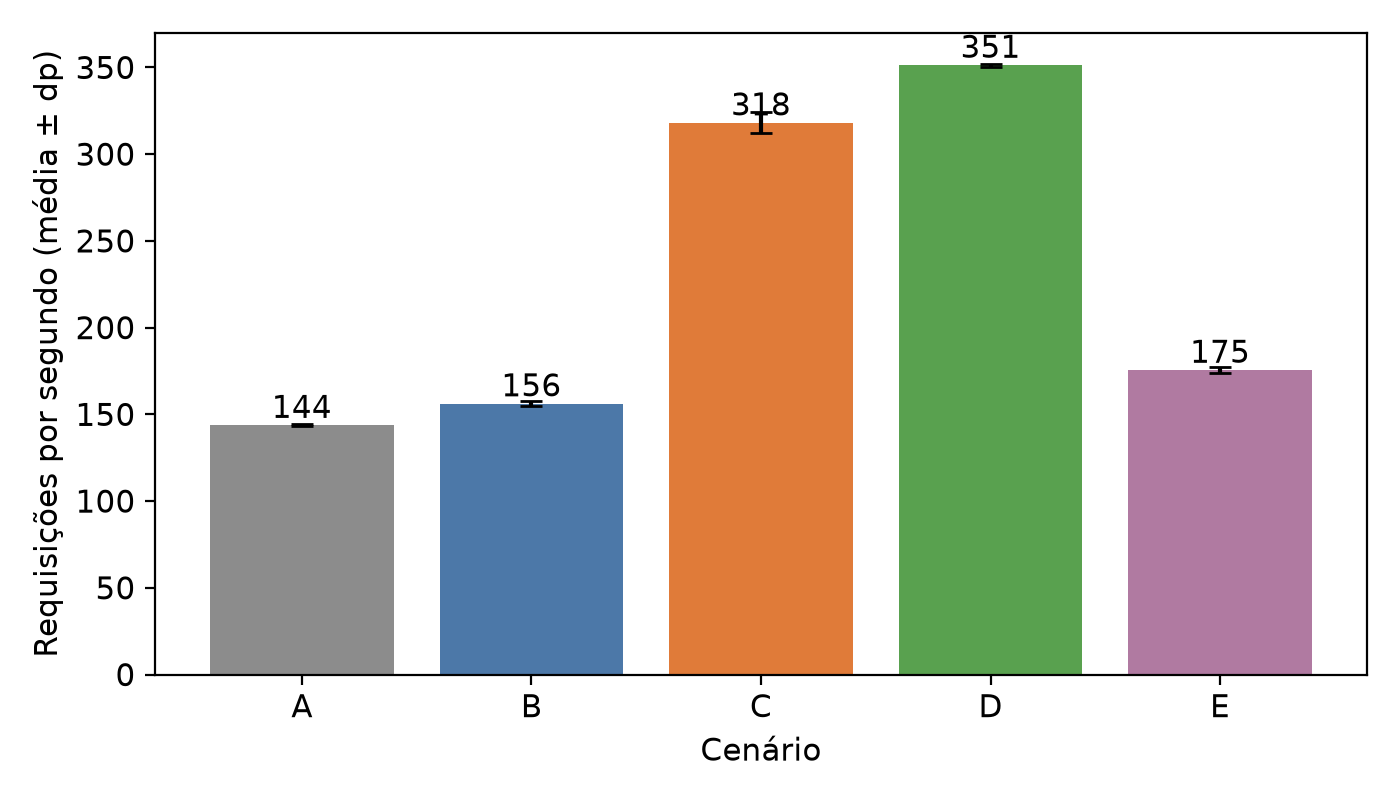
\includegraphics[width=0.92\linewidth]{figuras/fig_rps.png}
  \caption{Vazão média por cenário, com desvio-padrão de 3 execuções.}
  \label{fig:rps}
\end{figure}

Todos os cenários saturaram a CPU (92,7\% a 100,6\% de um núcleo, Figura~\ref{fig:rec}) e nenhum passou de 173~MiB de RAM, de modo que o gargalo é a CPU. A latência nos quatro \textit{endpoints} foi praticamente a mesma dentro de cada cenário: a latência média de \texttt{/db} (Tabela~\ref{tab:endpoints}) ficou apenas 1~ms acima da de \texttt{/health} em C e 2~ms em D, contra 36~ms em A e 43~ms em B, como mostra a Figura~\ref{fig:lat}, e a relação $N/X$ confere ($100/143{,}7\approx696$~ms contra p50 medido de 687~ms no cenário A; $100/318{,}1\approx314$~ms contra 300~ms em C).

\begin{table}[htb]
  \caption{Latência média por \textit{endpoint} (ms).}
  \label{tab:endpoints}
  \centering
  \footnotesize
  \setlength{\tabcolsep}{3pt}
  \begin{tabular}{lrrrr}
    \toprule
    \textbf{Cenário} & \textbf{/health} & \textbf{/compute} & \textbf{/memory} & \textbf{/db} \\
    \midrule
    A & 529,0 & 536,8 & 527,8 & 565,3 \\
    B & 482,2 & 492,1 & 484,2 & 525,4 \\
    E & 436,8 & 439,9 & 436,5 & 456,9 \\
    C & 241,3 & 251,1 & 241,3 & 242,2 \\
    D & 217,5 & 228,1 & 217,2 & 219,7 \\
    \bottomrule
  \end{tabular}
\end{table}

\begin{figure}[htb]
  \centering
  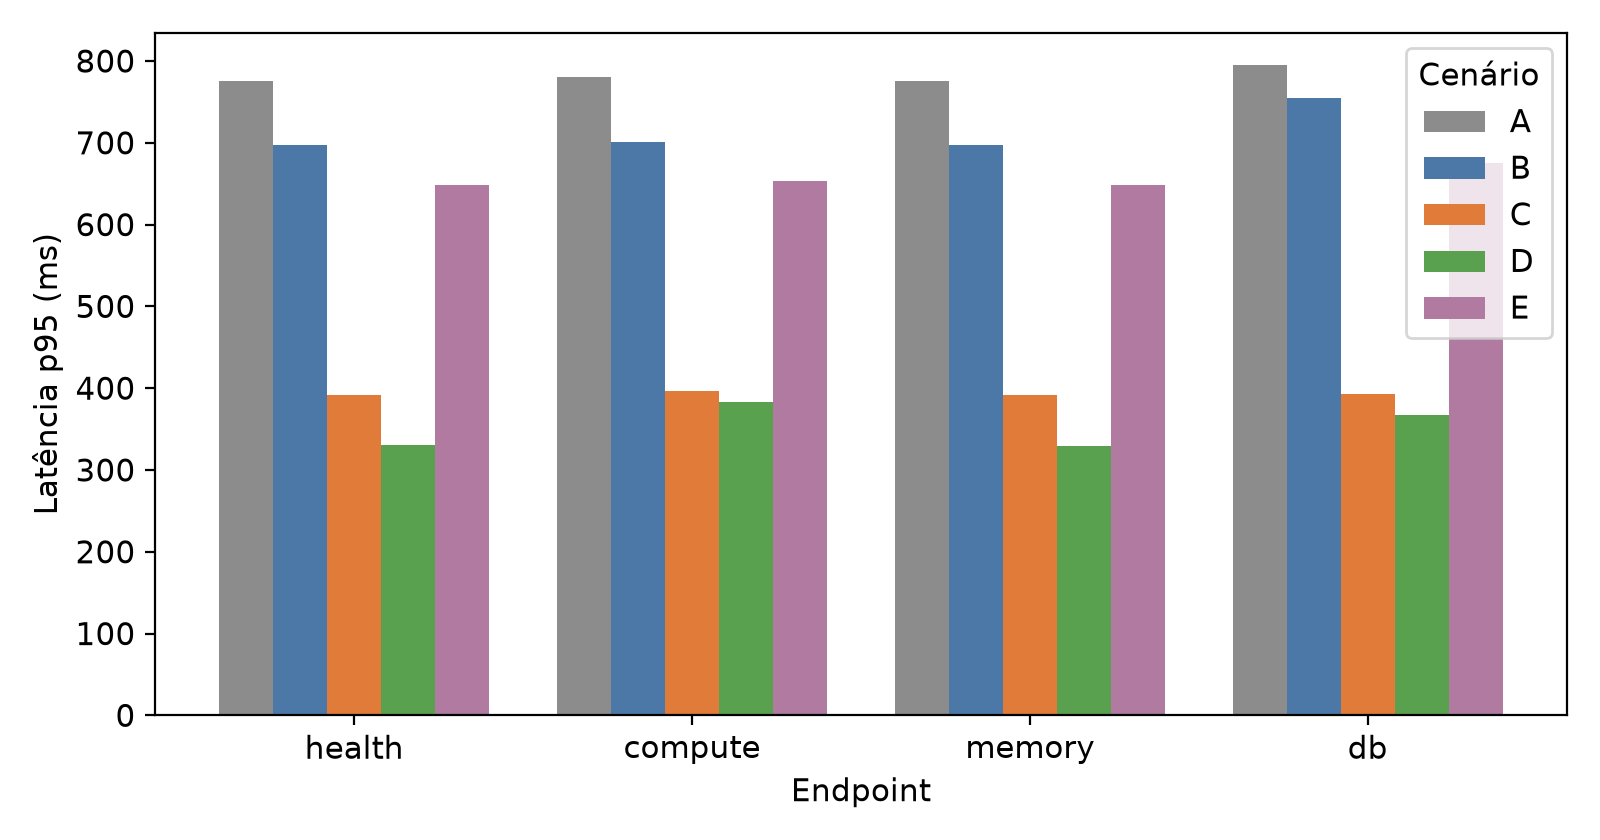
\includegraphics[width=0.95\linewidth]{figuras/fig_latencia_p95.png}
  \caption{Latência p95 por \textit{endpoint} e cenário.}
  \label{fig:lat}
\end{figure}

\begin{figure}[htb]
  \centering
  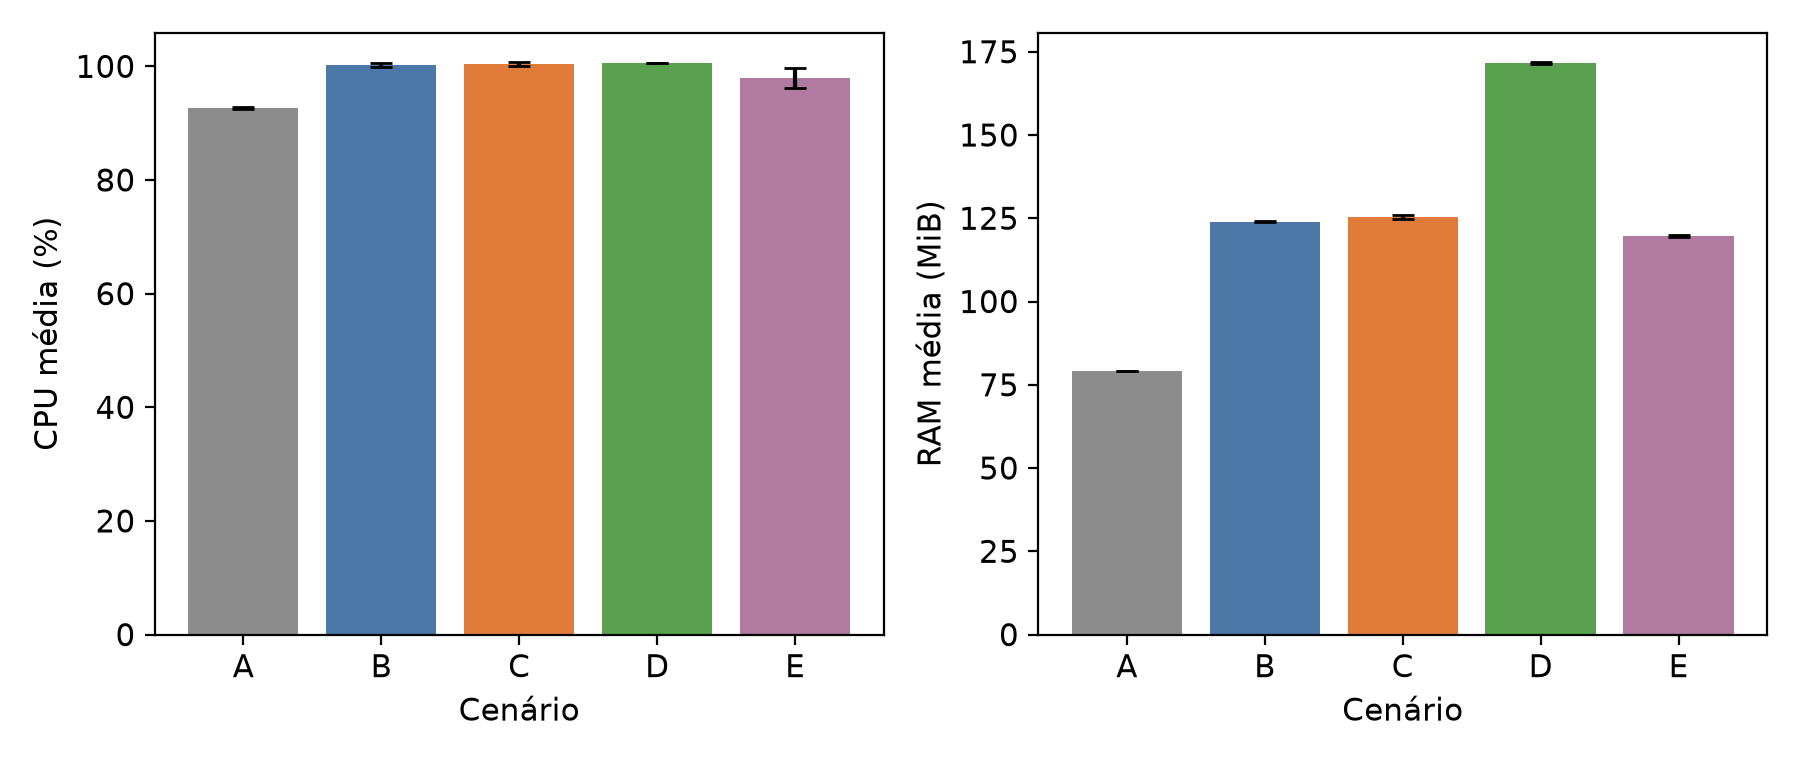
\includegraphics[width=\linewidth]{figuras/fig_recursos.png}
  \caption{CPU e RAM médias no patamar sustentado (3 execuções).}
  \label{fig:rec}
\end{figure}

O diagnóstico de persistência (Tabela~\ref{tab:estado}) mostra que C e D preservam o estado e a conexão com o banco por \textit{worker}, ao passo que A, B e E reiniciam ambos a cada requisição. Com um único \textit{worker}, 200 requisições sequenciais a \texttt{/memory} produziram um contador crescente de 2 a 201 e um único PID de conexão em C e em D; com quatro \textit{workers} e requisições concorrentes, o C usou quatro processos, cada um com seu contador e sua conexão. No D, o diagnóstico registrou um \textit{worker} adicional, coerente com o reciclo periódico de processos do Octane (cerca de 500 requisições), que não ocorreu no CI4. No teste de 30 minutos (Figura~\ref{fig:ram}), a RAM do C ficou em 125,8~MiB nos primeiros 5 minutos e em 126,0~MiB nos últimos, e a do D em 171,3 e 171,8~MiB; a vazão ficou 2,5\% (C) e 1,3\% (D) abaixo da das execuções de 15 minutos.

\begin{table}[htb]
  \caption{Estado preservado entre requisições.}
  \label{tab:estado}
  \centering
  \small
  \begin{tabular}{lll}
    \toprule
    \textbf{Cenário} & \textbf{Contador} & \textbf{Conexão com o banco} \\
    \midrule
    A, B, E & reinicia (sempre 1) & nova a cada requisição \\
    C, D    & cresce por \textit{worker} & mantida por \textit{worker} \\
    \bottomrule
  \end{tabular}
\end{table}

\begin{figure}[htb]
  \centering
  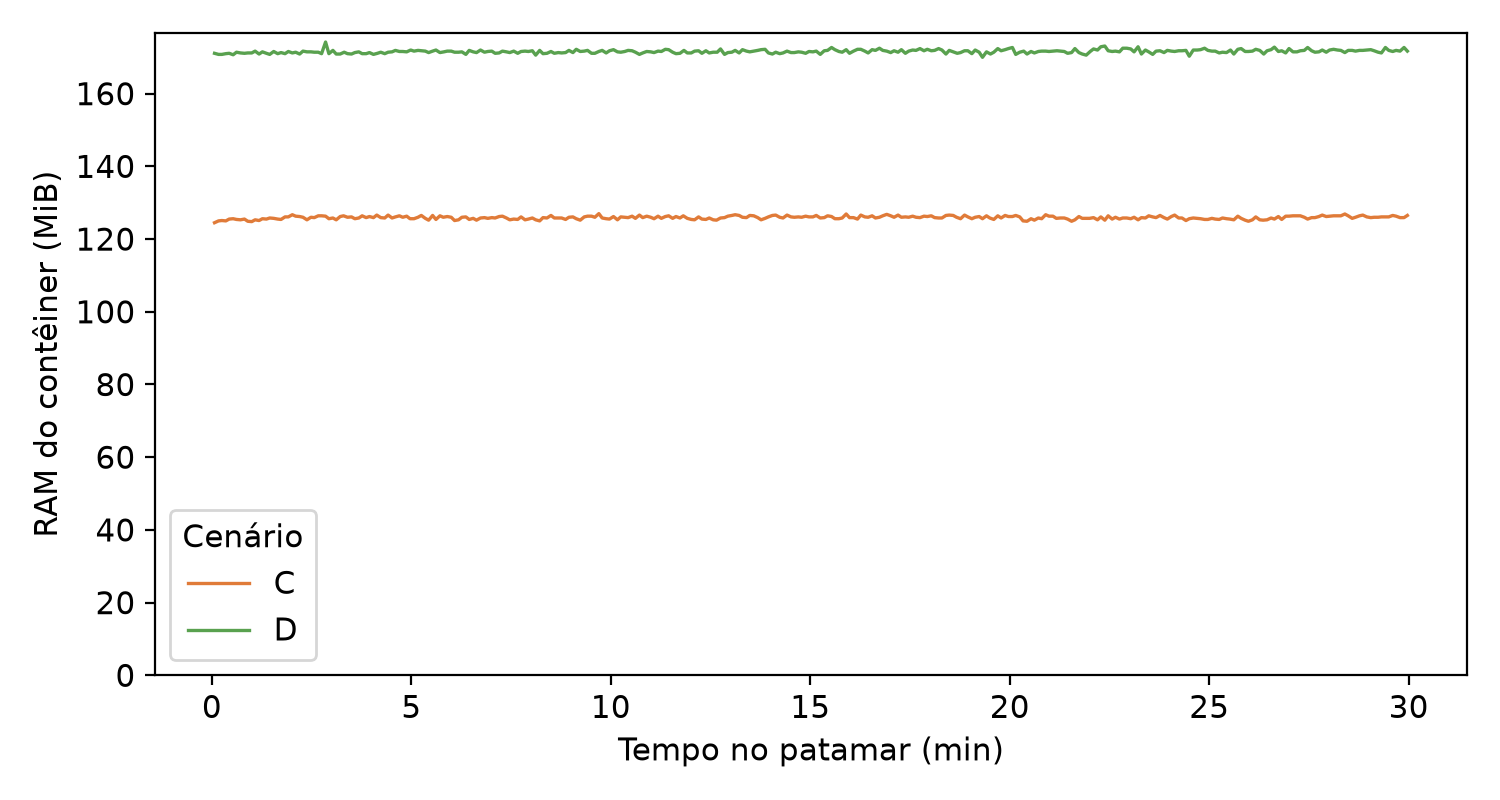
\includegraphics[width=0.92\linewidth]{figuras/fig_ram_longo.png}
  \caption{RAM dos contêineres C e D durante 30 minutos de patamar.}
  \label{fig:ram}
\end{figure}

\section{Discussão}
O resultado mais forte é que manter o processo e o \textit{framework} em memória mais que dobrou a vazão do CI4 e reduziu à metade o p95 e o p99 com os mesmos recursos, o que é coerente com o princípio do modo Worker~\cite{dungalas2024} e com a direção dos resultados de Luz et al.~\cite{luz2024} e Azzahidi et al.~\cite{azzahidi2025}. Como o CI4 em Worker preserva também a conexão com o banco, o ganho soma a eliminação do \textit{bootstrap} ao reaproveitamento da conexão; o experimento não separa as duas parcelas. O cenário B mostra que trocar apenas o servidor rende pouco, e o E indica que o modo clássico depende do número de \textit{threads}, mas mesmo assim fica 45\% abaixo do C: o ganho decorre do modo Worker, não do FrankenPHP em si.

Do ponto de vista de eficiência de recursos, o C processou 2,2 vezes mais requisições que o A com a mesma CPU e apenas 46~MiB a mais de RAM, o que significa menos instâncias para a mesma carga e se relaciona à busca por infraestrutura mais eficiente (ODS 9). Além disso, o cenário A foi o único que não saturou o núcleo (92,7\%), possivelmente porque a cota é dividida entre dois contêineres (PHP-FPM e Nginx) e a capacidade ociosa de um não pode ser usada pelo outro.

Esperava-se que o CI4, mais leve, superasse o Octane; ocorreu o contrário, com diferença pequena (10,4\% em vazão, sem significância após a correção) e menor uso de memória (125 contra 172~MiB). O Octane é um pacote maduro, projetado para esse modelo~\cite{otwell2024}, enquanto o suporte do CI4 é recente~\cite{codeigniter2024}; não houve perfilamento, e essas explicações são hipóteses. A estabilidade da memória em 30 minutos reduz a preocupação com vazamento, mas não a elimina para períodos mais longos ou aplicações complexas.

\subsection{Ameaças à validade}
Como limitações: execução em um único hospedeiro com o injetor na mesma máquina; carga sintética em modelo fechado, que torna a latência função da vazão; apenas três execuções por cenário, o que limita o poder estatístico; PHP \textit{thread-safe} no FrankenPHP e não no PHP-FPM; e imagens de monitoramento sem versão fixada.

\section{Conclusões e Trabalhos Futuros}
O modo Worker do FrankenPHP elevou em 121,4\% a vazão do CodeIgniter 4 sobre o PHP-FPM e reduziu a latência de cauda pela metade, ao custo de cerca de 46~MiB de RAM, com memória estável em 30 minutos e preservação de estado e conexão equivalentes às do Laravel Octane. Trocar apenas o servidor, mantendo o modo clássico, não justifica a migração pelo desempenho. Para equipes com aplicações em CI4, vale avaliar o modo Worker, observando a responsabilidade de evitar vazamento de estado entre requisições.

\subsection{Trabalhos Futuros}
Sugerem-se: carga de taxa de chegada fixa (modelo aberto) para isolar o custo de cada \textit{endpoint} e da conexão persistente; mais execuções por cenário; testes de várias horas com aplicações mais realistas, com sessões e consultas complexas; perfilamento para explicar a diferença entre C e D; e a comparação com Swoole e RoadRunner.

\section*{Agradecimentos}
Agradecimentos omitidos para fins de avaliação cega.

\section*{Declaração de Uso de Inteligência Artificial}
Foi utilizada a ferramenta de IA generativa Claude (Anthropic), por meio do Claude Code, como apoio na elaboração dos \textit{scripts} de automação da coleta e da análise estatística, na organização das tabelas e figuras e na redação e revisão textual deste trabalho. O autor definiu o desenho experimental, executou a coleta, conferiu os valores apresentados com os arquivos de resultados gerados pelos \textit{scripts}, revisou integralmente o conteúdo produzido e assume total responsabilidade pela precisão, originalidade e integridade científica do trabalho.

\bibliographystyle{ACM-Reference-Format}
\begin{thebibliography}{99}

\bibitem{azzahidi2025}
A. S. Azzahidi, B. Wijayanto, A. Darmawan. 2025. Performance Evaluation of Backend Frameworks for REST API: A Comparative Study of Spring Boot, Flask, Express.js, Laravel FrankenPHP, and Gin. \textit{Jurnal Teknik Informatika (JUTIF)} 6, 4 (2025), 2405--2419. \url{https://doi.org/10.52436/1.jutif.2025.6.4.4811}

\bibitem{brunst2022}
H. Brunst et al. 2022. First Experiences in Performance Benchmarking with the New SPEChpc 2021 Suites. arXiv:2203.06751. \url{https://arxiv.org/abs/2203.06751}

\bibitem{codeigniter2024}
CodeIgniter Foundation. 2024. \textit{CodeIgniter 4 User Guide}. \url{https://codeigniter.com/user_guide/}. Acesso em: 19 out. 2026.

\bibitem{dungalas2024}
K. Dunglas. 2024. \textit{FrankenPHP: The Modern Application Server for PHP}. \url{https://frankenphp.dev/docs/}. Acesso em: 19 out. 2026.

\bibitem{grafana2024}
Grafana Labs. 2024. \textit{k6 Documentation: Load Testing for Engineering Teams}. \url{https://grafana.com/docs/k6/latest/using-k6/metrics/}. Acesso em: 19 out. 2026.

\bibitem{jia2013}
Z. Jia et al. 2013. The Implications of Diverse Applications and Scalable Data Sets in Benchmarking Big Data Systems. arXiv:1307.7943. \url{https://arxiv.org/abs/1307.7943}

\bibitem{laaber2021}
C. Laaber, M. Basmaci, P. Salza. 2021. Predicting unstable software benchmarks using static source code features. \textit{Empirical Software Engineering} 26, art. 114 (2021). \url{https://doi.org/10.1007/s10664-021-09996-y}

\bibitem{little1961}
J. D. C. Little. 1961. A Proof for the Queuing Formula: $L=\lambda W$. \textit{Operations Research} 9, 3 (1961), 383--387. \url{https://doi.org/10.1287/opre.9.3.383}

\bibitem{luz2024}
J. M. da Luz, R. S. da Silva, C. D. Emer. 2024. \textit{Otimização de Aplicações Web com Programação Assíncrona em PHP e Swoole}. Instituto Federal do Rio Grande do Sul, Campus Avançado Veranópolis.

\bibitem{otwell2024}
T. Otwell. 2024. \textit{Laravel Octane Documentation}. Laravel LLC. \url{https://laravel.com/docs/13.x/octane}. Acesso em: 19 out. 2026.

\bibitem{zhan2022}
J. Zhan et al. 2022. A BenchCouncil View on Benchmarking Emerging and Future Computing. arXiv:2205.07769. \url{https://arxiv.org/abs/2205.07769}

\end{thebibliography}

\end{document}
